\documentclass{beamer}
\usepackage[utf8]{inputenc}

\usetheme{Madrid}
\usecolortheme{default}
\usepackage{amsmath,amssymb,amsfonts,amsthm}
\usepackage{tkz-euclide}
\usepackage{listings}
\usepackage{adjustbox}
\usepackage{array}
\usepackage{tabularx}
\usepackage{gvv}
\usepackage{lmodern}
\usepackage{circuitikz}
\usepackage{tikz}
\usepackage{graphicx}

\setbeamertemplate{page number in head/foot}[totalframenumber]

\usepackage{tcolorbox}
\tcbuselibrary{minted,breakable,xparse,skins}



\definecolor{bg}{gray}{0.95}
\DeclareTCBListing{mintedbox}{O{}m!O{}}{%
  breakable=true,
  listing engine=minted,
  listing only,
  minted language=#2,
  minted style=default,
  minted options={%
    linenos,
    gobble=0,
    breaklines=true,
    breakafter=,,
    fontsize=\small,
    numbersep=8pt,
    #1},
  boxsep=0pt,
  left skip=0pt,
  right skip=0pt,
  left=25pt,
  right=0pt,
  top=3pt,
  bottom=3pt,
  arc=5pt,
  leftrule=0pt,
  rightrule=0pt,
  bottomrule=2pt,
  toprule=2pt,
  colback=bg,
  colframe=orange!70,
  enhanced,
  overlay={%
    \begin{tcbclipinterior}
    \fill[orange!20!white] (frame.south west) rectangle ([xshift=20pt]frame.north west);
    \end{tcbclipinterior}},
  #3,
}
\lstset{
    language=C,
    basicstyle=\ttfamily\small,
    keywordstyle=\color{blue},
    stringstyle=\color{orange},
    commentstyle=\color{green!60!black},
    numbers=left,
    numberstyle=\tiny\color{gray},
    breaklines=true,
    showstringspaces=false,
}
\usepackage[utf8]{inputenc}
\usepackage[T1]{fontenc}



%------------------------------------------------------------
%This block of code defines the information to appear in the
%Title page
\title %optional
{1.2.11}
\date{August 21,2025}
%\subtitle{A short story}

\author % (optional)
{Megha Shyam-AI25BTECH11005}
\begin{document}
\begin{frame}{question}
Find the values of $k$ for which the points $A(k+1, 2k)$, $B(3k, 2k+3)$, $C(5k-1, 5k)$ are collinear. 
\end{frame}
\begin{frame}{Theoritical solution}
    First, form the difference vectors:
\[
 B - A = 
\begin{pmatrix}
3k - (k+1) \\ (2k+3) - 2k
\end{pmatrix}
=
\begin{pmatrix}
2k - 1 \\ 3
\end{pmatrix}
\]
\[
 C - A =
\begin{pmatrix}
(5k-1) - (k+1) \\ 5k - 2k
\end{pmatrix}
=
\begin{pmatrix}
4k - 2 \\ 3k
\end{pmatrix}
\]

Form the matrix:
\[
M = \begin{pmatrix}
2k-1 & 3 \\
4k-2 & 3k
\end{pmatrix}
\]

For the points to be collinear, the rank of $M$ must be $1$. Perform the row operation:
\[
R_2 \to -\frac{4k-2}{2k-1}R_1 + R_2 \qquad \text{(for $2k-1 \neq 0$)}
\]

Which gives:
\[
\begin{pmatrix}
2k-1 & 3 \\
0 & 3k - \frac{3(4k-2)}{2k-1}
\end{pmatrix}
\]
\end{frame}
\begin{frame}{Theoritical solution}
    

Set the second row entry to zero for rank $1$:
\[
3k - \frac{3(4k-2)}{2k-1} = 0
\]
\[
3k = \frac{3(4k-2)}{2k-1}
\]
\[
3k(2k-1) = 3(4k-2)
\]
\[
6k^2 - 3k = 12k - 6
\]
\[
6k^2 - 15k + 6 = 0
\]
\[
2k^2 - 5k + 2 = 0
\]

Solving for $k$:
\[
k = \frac{5 \pm 3}{4}
\]
\[
k = 2 \quad \text{or} \quad k = \frac{1}{2}
\]


\end{frame}
\begin{frame}[fragile]{C code}
\begin{lstlisting}[language=C]

int areCollinear(double Ax, double Ay, double Bx, double By, double Cx, double Cy) {
    double BA_x = Bx - Ax;
    double BA_y = By - Ay;
    double CA_x = Cx - Ax;
    double CA_y = Cy - Ay;

    if (BA_x * CA_y == BA_y * CA_x) {
        return 1;  // Points are collinear
    } else {
        return 0;  // Points are not collinear
    }
}


\end{lstlisting}
\end{frame}



\begin{frame}[fragile]

\frametitle{\textbf{Python Plotting Code - Part 1}}
\begin{lstlisting}[language=Python]
import matplotlib.pyplot as plt
import numpy as np
# Part 1: Define points for each k and plot points
k_values = [0.5, 2]  # values of k for collinearity
plt.figure(figsize=(8,6))
for k in k_values:
    A = np.array([k+1, 2*k])
    B = np.array([3*k, 2*k+3])
    C = np.array([5*k-1, 5*k])
     plt.scatter(*A, color='red')
    plt.scatter(*B, color='green')
    plt.scatter(*C, color='blue')
     plt.text(A[0], A[1], 'A', fontsize=12, color='red', ha='right')
    plt.text(B[0], B[1], 'B', fontsize=12, color='green', ha='right')
    plt.text(C[0], C[1], 'C', fontsize=12, color='blue', ha='right')
\end{lstlisting}
\end{frame}
\begin{frame}[fragile]

\frametitle{\textbf{Python Plotting Code - Part 2}}
\begin{lstlisting}[language=Python]
    x_line = np.linspace(min(A[0], B[0], C[0])-1, max(A[0], B[0], C[0])+1, 100)
    y_line = ((B[1]-A[1])/(B[0]-A[0])) * (x_line - A[0]) + A[1]
    plt.plot(x_line, y_line, label=f'Line through A and B for k={k}')

plt.title('Collinearity of Points A, B, C for values of k')
plt.xlabel('x')
plt.ylabel('y')
plt.legend()
plt.grid(True)
plt.show()


\end{lstlisting}
\end{frame}
\begin{frame}[fragile]
\frametitle{plot}

\begin{figure}
    \centering
    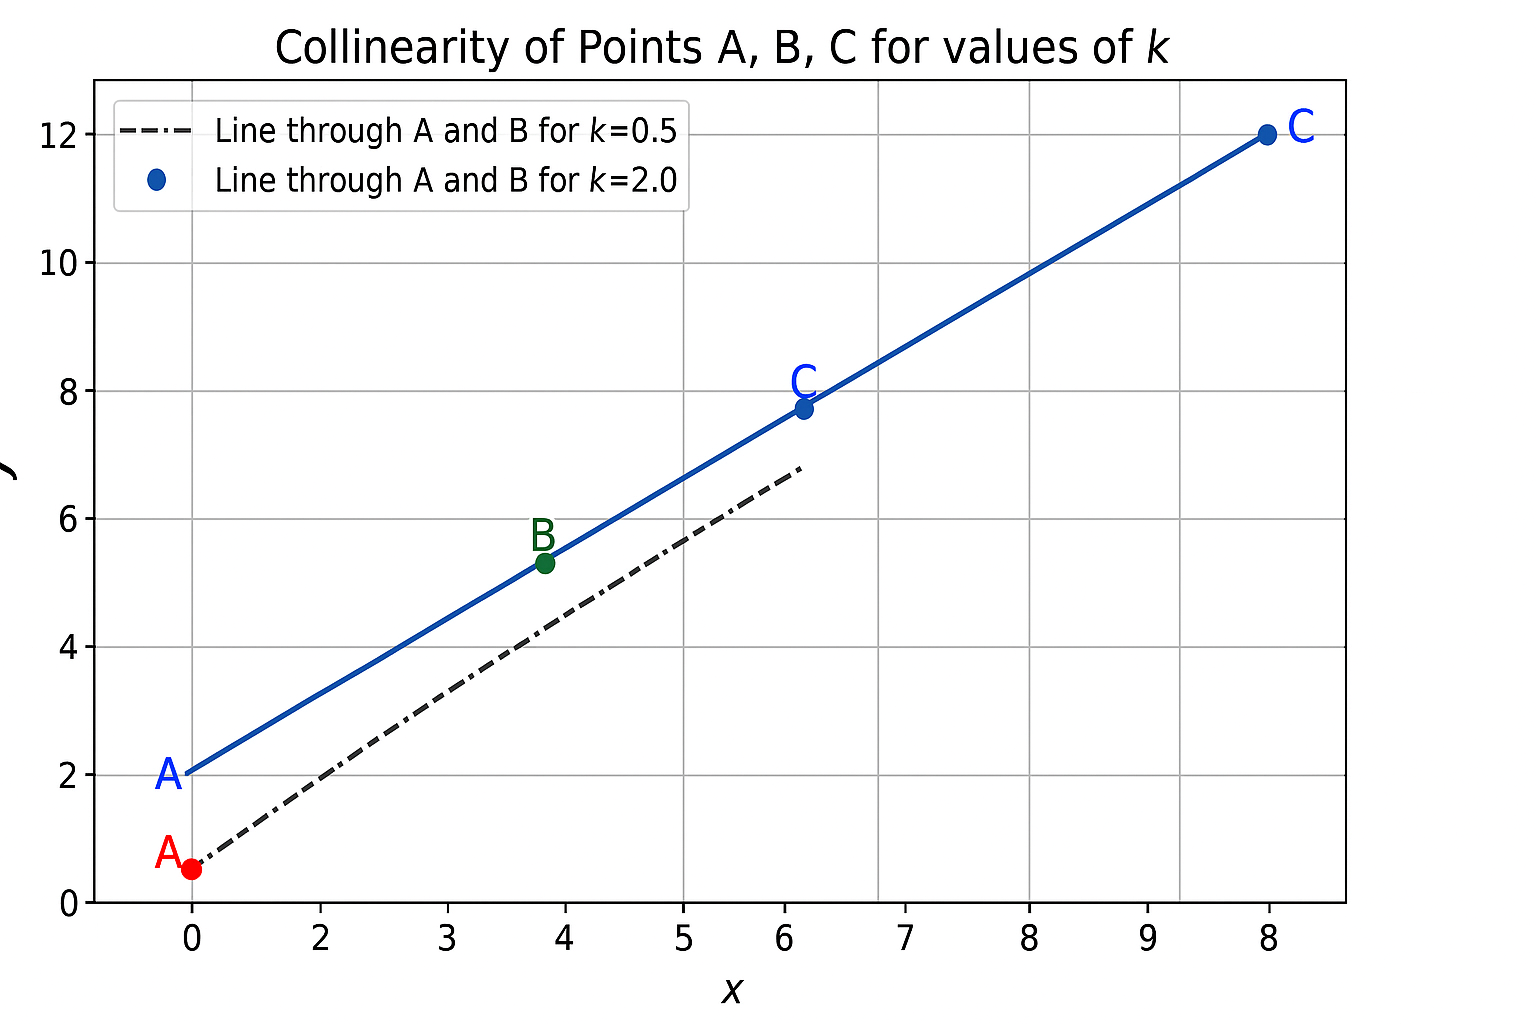
\includegraphics[width=0.5\linewidth]{figs/plot.png}
    \caption{collinear}
    \label{fig:placeholder}
\end{figure}



\end{frame}


\end{document}




